\label{sex:sex}
\index{Sex|(}
\renewfontfamily\pagenumfont{Gentium Book Basic}[Color=111111FF]

\backgroundcolor{c[0]}[HTML]{eeeef8}
\backgroundcolor{C[0](10000pt,10000pt)(0.6\columnsep,10000pt)}[HTML]{eeeef8}
\backgroundcolor{c[1]}[HTML]{eeeef8}
\backgroundcolor{C[1](0.6\columnsep,10000pt)(10000pt,10000pt)}[HTML]{eeeef8}

\begin{paracol}{2}
\begin{leftcolumn}

\fontspec{Gentium Book Basic}[Color=111111FF,Ligatures=TeX]
\renewfontfamily\allyFont{Merriweather Sans}[Scale=0.9,Color=333333FF,Ligatures=TeX]

\noindent Cathleen Schine writes in \emph{The Evolution of Jane}:

\begin{quotation}
  \noindent I resented the state of childhood wonder.  It was insatiable, yet it seemed to me to be no more than a puerile affliction, like baby teeth.  My ignorance struck me as a bizarre anomaly, for I felt, with utter certainty, that I was --- how can I say this? --- that I was *sufficient*.  Evidence to the contrary forced itself on me every hour of every day, but that seemed to me some preposterous misunderstanding.
\end{quotation}
And while I don't necessarily have fond memories of childhood--

\begin{ally}
Clearly not
\end{ally}
--some part of me does rather miss the childlike curiosity with which I was able to approach sexuality early in puberty. It was all so abstract and confusing. Every time I'd try something new, there would be this thrill of danger, this rush of excitement. The lone copy of \emph{Joy of Sex}'s assurances aside, was each burst of pleasure actually something going \emph{horribly wrong?}

\begin{ally}
Ah, to be young and anxious.
\end{ally}
And I really was. Like many kids, I suspect, my first orgasm was terrifying. I thought I'd broken myself.

\begin{ally}
You got over it.
\end{ally}
Boy did I. I soon learned to love masturbation.

But still, the bit I yearn for was the utter simplicity of my explorations. There was a lot of \emph{does this feel good} and \emph{let's try this} and so on, as I spent hours just trying to figure out what the hell bodies even are.

\begin{ally}
And the best part of it all is that it didn't involve anyone else. Your fantasies were about feeling good, or perhaps about some vague idea of sex as a concept, but it was all so abstract. The orgasm --- later, the delaying of such --- became the highest goal, the purest art. Other people just got in the way.
\end{ally}
It was a bit telling, wasn't it?
\newpage

\noindent How can one be sexual when the act of engaging in sex is so confusing, so anxiety-inducing as to be not worth it no matter how barked up one is?

\begin{ally}
You're getting ahead of yourself. The solutions arrived before the problem made itself known.
\end{ally}
I suppose so.

My first sexual experiences took place over the phone and over text. Late night, parked in front of my computer with the cordless pinned between my cheek and shoulder, Danny and I masturbated together 1,800 miles apart. There was only the soft sounds of breathing, the quiet monosyllables, and the rushed reassurances that, yes, we were close, and then a shaky sigh from both of us.\index{Relationships!Danny}

\begin{ally}
You can still hear his voice saying two things: ``Mattie'', his pet name for you, and the sleepy, giddy kind of ``I love you'' that comes after an orgasm when you've both stayed up far too late.
\end{ally}
I only met him once. We just smoked weed together in a hotel bathroom, hung out, cuddled. Sex would be too complicated for us, by then. We had gone our different ways. We had become different people.

\begin{ally}
And by then, you'd started encountering the aforementioned problem.
\end{ally}
Yes.

Another easy solution I latched onto was erotic roleplay. TS. Typefucking. Co-authoring erotica.

I latched on and wouldn't let go. Still haven't. Beyond even myself, it shows up in my writing:

\index{Writing!samples!fiction|(}
\begin{quotation}
  \noindent And it was there where I found love. There where I found love and lust and romance and flings. I dated. I TSed (we were, of course, too cool to use so vulgar a word as ‘cyber’). I set up relationships for characters in our games, and I set up relationships that transcended that, two hearts touching through only those white words on a black screen.

  Merlin and Marusin, The\_Prof and rranger386, people I would dream about and likely never meet. We were all young. We were in love with each other in our own little worlds, serially and in parallel.

  And while sometimes I would think about who they were beyond the screen, it was rarely for long. I was in love with Merlin the fighter who hated magic. I was in love with The\_Prof the student who desperately wanted to be a professor when he grew up, and didn’t care which subject.

  Sometimes I would think about who they were when we TSed, would wonder what it would be like to have their paw instead of my own around my erection, but never for long. It was easier. It was safer to not bother with it.

  But our relationships were as real as any collocated flings. More so, we told ourselves, for the purity of essence that came with no flesh to get in the way.

  I’m sure we all hungered for touch.
\end{quotation}
\index{Writing!samples!fiction|)}

\begin{ally}
Did you?
\end{ally}
Did I what? Write bits of my life into furry fiction?\index{Furry}

\begin{ally}
Hunger for touch.
\end{ally}
In some cases, sure. I wanted nothing more than to hold, to be held. I wanted nothing more than to experience arousal and climax with these people I loved.

\begin{ally}
And that was the problem.
\end{ally}
Yes. The problem was that I wanted to experience arousal and climax, but not really the whole sex part. Or perhaps I wanted that frictionless sex that can be accomplished in typefucking. I wanted that consequence-free, painless, perfectly-lubricated and utterly mess-less sex.

Even then, I'm not so sure.
\newpage
\index{Sex!asexuality|(}
\noindent The problem was that I didn't really want sex. I loved the idea of it, loved reading and writing about it, loved ERP, loved consuming art, loved thinking about it, loved masturbating. I just didn't really love sex itself.

Not for lack of trying, mind. I played around with my partners, tamping down my anxiety and squeamishness in order to try and just enjoy myself, enjoy our times together. Often, I was at least reasonably successful, too. I still have fond memories of some fun romps.

\begin{ally}
What rankled?
\end{ally}
It was a few things, I think. The most obvious being the increasing dissonance between my body and my identity as `male' started to fit less and less. When having a penis seems odd and discordant, engaging with it feels unsatisfactory at best, nauseating at worst.

Another was simply the mess of it all. Water-based lube gets sticky. Condoms are finicky. Fluid-bonding is great, but then the mess is magnified. Foreskin is complicated --- a rough weekend of too much masturbation left me scarred, the resulting phimosis making sex something of an adventure.

I think, most often, it was just that it was a lot of work. You had to set aside time. You had to negotiate. You had to have the condoms handy. You had to have the lube handy. You had to both be willing and on the same page. All perfectly doable, but whether or not it was worth it was something that seemed to vary from day to day.

\begin{ally}
And the shame.
\end{ally}
Yes, there was plenty of that. The unswerving sense that I had messed up. That I was doing something wrong. That this was all so disgusting. That this baffling act of smashing meat together was somehow a positive thing, but I just couldn't see how.

\begin{ally}
You tried to cleanse yourself of that with TIASAP.\index{Gender!TIASAP} You also tried going the other way. You went to the Underground parties. You gathered around you a core group of people you trusted and played with them. You worked to extract that shame from yourself so that you could live without it.
\end{ally}
Sometimes it worked. Sometimes it was a matter of the stars aligning.

Of those fond memories I mentioned, most of them surround lazy, comfortable sex, where everything was just aligned. Giving a cozy blowjob on a couch with no time pressure. Putting my hair up with a chopstick. That Underground party with lube and condoms readily available, and us two incidentally parked near enough that getting started was no stress. Sneaky fingers slipping past elastic waistbands. Tentative touches.

\begin{ally}
Sex that you had for fun. Sex with people you were close to. Sex with no expectations.
\end{ally}
Which I suppose is how it should be, but that rarely seems to be the case. Even when JD and I had moved in together and were sexually active, it was often more stress than it was worth.

\begin{ally}
And then you gave up trying to conquer shame.
\end{ally}
Yes. And since, by that point, every sexual act I engaged with left me feeling awful, I effectively gave up on sex.
\newpage

\begin{ally}
Where did the shame come from?
\end{ally}
I'm not sure. I've got a few ideas, though.

The first is likely that, as a queer person, societal shame is just part of our lives. We're not normal, after all. The sex we have doesn't line up with the sex we \emph{should} have.

I certainly bought into that, despite all of my efforts. Homosexual stuff was fine online, of course, because it was all so idyllic and perfect. No muss, no fuss. To be confronted with just how much of a mess sex can be offline, especially between two bepenised individuals, left me feeling like somehow I was falling short of that ideal.

\begin{ally}
Perhaps that is the crux of the shame: sex should be easy, and you should be good at it, if your online sex life was anything to go by. That it isn't and that you aren't felt like an indictment.
\end{ally}
Yes. The second idea that I have is that there was that misalignment between body and mind that started in 2005 and just grew wider over time. This put that indictment in very stark terms: sex should be easy, I should be good at it, and I should be a girl, if my online sex life was anything to go by, and I was none of those things.

\begin{ally}
Has the shame lessened since transition? Since surgery?
\end{ally}
Oh, quite a bit. I still feel like I'm not very good at it, that it's not easy, but I no longer have that overwhelming sense that I'm lying to everyone I lay with.

\begin{ally}
Your other ideas?
\end{ally}
Two. The first is subtler, and more of a subset of stuff already mentioned. To be raised a boy in America in the 90s is to be raised with the competing ideas that women are people and that women are sexual objects. Having sex is a balancing act between claiming what is rightfully yours as a man and treating a woman right.

To then be gay, and especially then to bottom, is to turn every bit of that on its head. You become the sexual object. You become the person who should be treated right. You fulfill all these obligations placed on sex, but somehow manage to do so completely wrong. You fuck it all up.

\begin{ally}
The other?
\end{ally}
Getting raped just kind of messes you up.\index{Sex!rape}

\begin{ally}
Ah.
\end{ally}
So, let's talk about kink.

\newpage
\end{leftcolumn}
\end{paracol}

\renewfontfamily\pagenumfont{Gentium Book Basic}[Color=EEEEEEFF]

\backgroundcolor{c[1]}[rgb]{0.0902,0.0667,0.102}
\backgroundcolor{C[1](0.5\columnsep,1000pt)(10000pt,10000pt)}[rgb]{0.0902,0.0667,0.102}

\begin{paracol}{2}
\begin{rightcolumn*}
What do you do when you've got a libido and relatively little will to act upon it?

Delve into kink.

\begin{ally}
Well, and fuck around on Taps a lot.
\end{ally}
The two go hand in hand. When sex makes you intensely anxious, it turns out that getting tied up and blindfolded just sort of multiplies that anxiety.

\begin{ally}
So you removed yourself from the equation.
\end{ally}
Close enough, yes. I let my characters bear the weight of kink and sexual interaction. Textually, there's a vast divide between what's on the screen and what's going on in person. I can get all I need from kink without actually needing to interact with it.

\begin{ally}
And what do you need from kink?
\end{ally}
Beyond just fantasy fulfillment? A way to cope, I suppose.

\noindent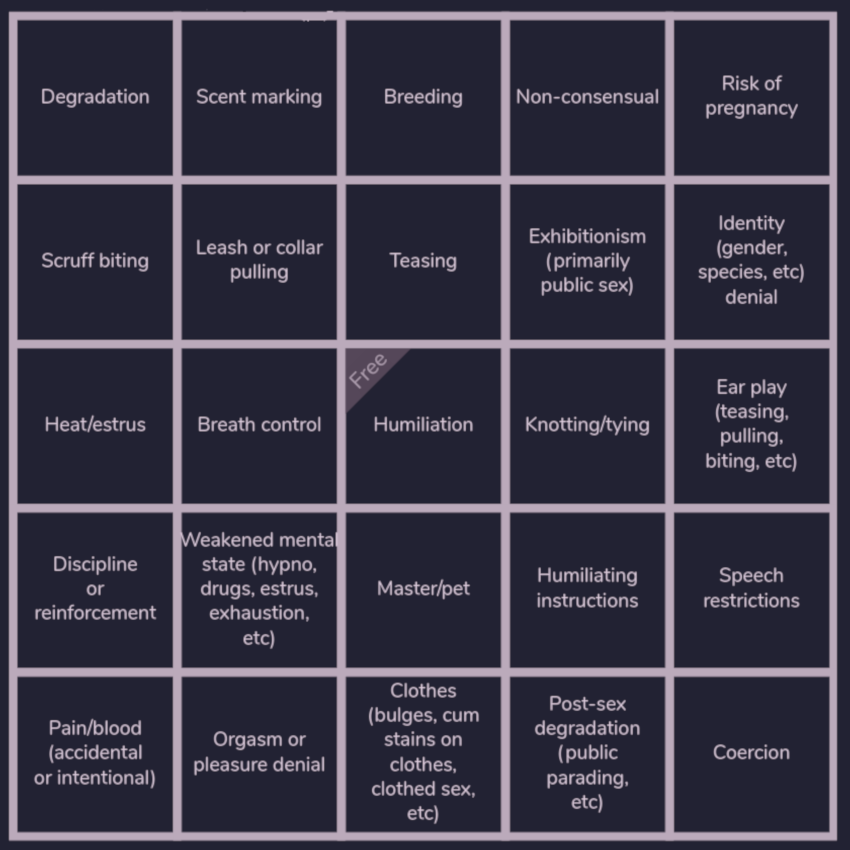
\includegraphics[width=2.5in]{assets/static/sex/kink/bingo.png}

\begin{ally}
I'm not really sure what to make of the fact that you made a bingo card for your kinks.
\end{ally}
Well, hey, hit bingo, and maybe I explode or something. Besides, \href{https://bbbingo.me}{bbbingo} was for a game jam.

\begin{ally}
So tell me about your free space.
\end{ally}
Actually, I think many of them come from a similar space: recasting bad or uncomfortable experiences from childhood into some positive light. A way to reclaim them and make them positive again.

\begin{ally}
How is humiliation positive?
\end{ally}
Okay, maybe some of them are not so much `again'.

\begin{ally}
I don't imagine non-consensual sex ever was, no.
\end{ally}
Not really, but using kink as a coping mechanism for anxieties around rape is at least a way forward for me.

Ditto humiliation. Being made to feel inadequate, often by people I was supposed to look up to, was such a negative force in my life --- in Matthew's life --- that it left me with quite a bit of baggage. This is just a way to sort through it.

\begin{ally}
Sexily.
\end{ally}
I suppose. It's something of a metakink. Many of the others stem from that, or from a similar core interest.

Scent-play as a means of degradation: why would a snow leopard smell of canine? Fits in nicely with knotting. Why not toss in some species denial, too; no more kitty, you say `arf' now.

Scruffing, in the context of furry, especially with felines, is a means of rendering one helpless. Coercion and weakened mental states fit as well. Those all sort of tag along with the non-consensual core kink

\begin{ally}
So, pain and blood? Breathplay?
\end{ally}
Yes. Abuse. Damage. Bad ends.

\begin{ally}
Where do those come from?
\end{ally}
Self hatred. Self harm. Destroy me before I destroy myself.

\begin{ally}
Really?
\end{ally}
No, of course not.

\begin{ally}
But some part of you actively believes that? Some part of you actively craves someone destroying you? Beating you bloody? Choking you? Leaving you for dead with casual nonchalance?
\end{ally}
Yes.
\newpage

\begin{ally}
Do you enjoy vanilla sex, then?
\end{ally}
Perhaps. I suppose I must. So much of what I did for so long, online and off, was vanilla. Even now, much of it is.

\begin{ally}
Yet ``sneps are for abusing''.
\end{ally}
Yes.

\begin{ally}
Why?
\end{ally}
I enjoy vanilla sex. It feels good. All this kink, though, helps me grow. It's exposure therapy.

It was exposure therapy when a TS partner on Taps laughed in my face as he raped me and left me to clean myself up. It is exposure therapy because I can say no, because I can enjoy being tied up now.

It was exposure therapy when I was ordered to describe what I wanted in lurid detail. It's exposure therapy because I can talk about sex now.

It was exposure therapy when I entered into a few master/pet relationships. It's exposure therapy because at some point I was able to handle a power-dynamic in my relationships.

It was exposure therapy when I spent scene after scene toying with fertility. It's exposure therapy because at some point I was able to deal with the idea of not being cis, of motherhood being unattainable.

It was exposure therapy when I made my character a pudgy nerd and still able to engage with her sexually. It's exposure therapy because I've been able to come to terms with my body.

\begin{ally}
It's exposure therapy because at some point, you started enjoying sex --- or at least enjoying it more --- and the thought of sharing that with someone.
\end{ally}
Yes.
\newpage

\end{rightcolumn*}
\begin{leftcolumn}
  \null
  \newpage
\noindent I can't let this go.

\begin{ally}
Why not?
\end{ally}
I just can't. I doubt it's possible, but I need to somehow get this off my chest. I need to be able to throw enough words at it that it leaves me alone. I need\ldots{}not a solution, but perhaps some sense of closure, of having explained it well enough that I may be forgiven.

\begin{ally}
Forgiven what? Your trespasses? Your sins?
\end{ally}
Perhaps. Perhaps I need to be forgiven my inadequacies.

\begin{ally}
Explain away, then.
\end{ally}
I spend a lot of time walking circles around the concept of asexuality. It's an uncomfortable thought, an identity that itches for someone who feels attraction, who otherwise enjoys the idea of sex, is capable of even enjoying the act.

\begin{ally}
So long as it doesn't actually involve you.
\end{ally}
Yes.

Autochorissexualism, they call it, though the word is clunky to the point of inoperable. The feeling of being generally positive on sex to the point of getting turned on, so long as it doesn't actually involve oneself. Fictional characters, visual art, and text-based role-play seem to be the bailiwick of such.

I suppose, if you spend so much time feeling a fundamental disconnect from your body, such an identity is almost bound to form. Even before I felt so plagued by dysphoria that interacting sexually was problematic in its own right, even before I was able to engage with another person sexually in, as it were, the flesh, I was embedded in long distance relationships where sexual interaction was based on the idea of sex rather than the actual practice of it.

\begin{ally}
Was that a choice?
\end{ally}
I don't know. I suppose, on some level, it was. Could I have dated someone local instead of Danny? Instead of Marek or Andrew? Sure, I guess.

\begin{ally}
But you didn't.
\end{ally}
No.

\begin{ally}
Why not?
\end{ally}
I suppose that would have required me coming out to my parents more formally. Or, perhaps, it would've required me gaining a level of sneakiness in my social interactions that I don't think I'm really capable of.

Not only that, but I dove into furry halfway through puberty, and I dove in \emph{hard}. It was my distraction from a shitty few years of life, from a shitty entry into puberty. And, with the whole running away fiasco, the sudden moving of schools, it was my whole social circle.

And hey, one dates within one's social circle, right? That would require having a local furry scene.

\begin{ally}
You had Shannon and Ash.
\end{ally}
Well, yes, but Ash and I had known each other since second grade. Something about it didn't feel right. And this is back when I was very, very gay. For better or for worse, Shannon and I were not relationship material.

\begin{ally}
Had you been more open to dating women, do you think you would have been?
\end{ally}
Perhaps. I don't know how long that would have lasted, though, had we gone in that direction. After a time, we simply became better friends material than we would have made relationship material.

\begin{ally}
There was Pilot.
\end{ally}
We were in no way compatible.

\index{Relationships!Michael|(}
\begin{ally}
There was Michael.
\end{ally}
I \emph{knew} it. I knew that was coming. I could feel you winding up to throw that in my face.\index{ally!throwing stones}
\newpage

\begin{ally}
So, tell me about Michael in a second, but tell me why you knew that was coming.
\end{ally}
Why should I? We both know.

\begin{ally}
Because it's important that you be able to contextualize this discussion.
\end{ally}
It was the order of your questions. It was the way you came at things so circuitously. It was the way you asked about the local furry scene specifically without mentioning him. It's the way you nudged me about Shannon before bringing him up.

\begin{ally}
Was that uncouth?
\end{ally}
A little. Ask about relationships as relating to a woman, then ask me about when I started dating a trans man. Are you my internalized transphobia?

\begin{ally}
Not my department. You hate yourself far more than this conversation entails.
\end{ally}
Of course.

\begin{ally}
Still, the answer is no. I do not ask about him out of some weird sense of transphobia, so much as because, with Shannon, you mentioned being very, very gay, and yet your relationship with Michael was still sexual.
\end{ally}
So?

\begin{ally}
There is an aspect of biology here that needs mentioning.
\end{ally}
Or at least talking around in circles.

\begin{ally}
No, mentioning. You went into your relationship with him gay to the point of describing your aversion to vaginas, and you came out of it solidly bi despite him being a man.
\end{ally}
Point.

\begin{ally}
Yes.
\end{ally}
Our relationship was indeed sexual. It didn't involve PiV sex until it was no longer a romantic relationship, but there's no denying the that aspect of it. There's no denying the attraction, even if at the time, I chalked it up to him being transmasculine.

\begin{ally}
Was there perhaps some aspect of \textbf{doppelwunsch} to it? Some bit of ``I don't know whether I want to be with him or be him''?
\end{ally}
If so, it was only the tiniest shadow of a prelude. We dated when I was seventeen and eighteen. I didn't really do the whole \emph{gosh, maybe I'm trans} thing until I was in my mid twenties.

\begin{ally}
Hindsight is 20/20.
\end{ally}
I hate that phrase.

\begin{ally}
2016: ``I think''hindsight is twenty-twenty" is better reserved for cases when seemingly unrelated occurrences come together to form an outcome that seems to be greater than the sum of the parts. It fits best when you look back at your life and see disparate, unconnected events come together to make the situation you find yourself in now."
\end{ally}
\end{leftcolumn}
\end{paracol}

\backgroundcolor{c[1]}[rgb]{0.2,0,0}
\backgroundcolor{C[1](0.5\columnsep,1000pt)(10000pt,10000pt)}[rgb]{0.2,0,0}
\begin{paracol}{2}
  \begin{rightcolumn*}
    \fontspec{Gentium Book Basic}[Color=DCCCCCFF,Ligatures=TeX]
\renewfontfamily\allyFont{Merriweather Sans}[Scale=0.9,Color=CBBBBBFF,Ligatures=TeX]

\begin{ally}
Tell me about rape.
\end{ally}
No.

\begin{ally}
Talk in circles around it, then, and then tell me why you won't tell me about it. Or vice versa. I don't care. I'm not picky as to the order.
\end{ally}
Fine.
\newpage

\noindent Let's say, as we have already, that you spend much of puberty up in your head, and then when you start branching out into engaging sexually with others, you do so in a purely intellectual way. One which involves some sort of platonic ideal of sexuality. You never feel awkward. Everything always just works.

Let's just take that for granted.

Let's also take for granted that this mechanism of interaction is one wherein getting out of a sexual interaction that is uncomfortable, or pressured, or hell, even nonconsensual is a matter of just\ldots{}stopping. Come up with an excuse. Come up with some lie. Eschew the truth in favor of making the other person happy, as you would your father.

\begin{ally}
That's not possible. Being pressured into typefucking is just as easy as it is to be pressured into sex in the embodied world.
\end{ally}
I'll agree with that. Take it for granted, then that this is what you believe. You believe that consent is implicit in the act, because to revoke consent is as simple as signing off or pretending that your parents walked in on you.

\begin{ally}
Okay.
\end{ally}
Now take the type of person who takes all that for granted, and put them in a situation with someone who has an overbearing personality, who gets what they deserve, and who deserves you. Take that type of person and put them in a situation where sex is expected of them.

What do you suppose happens?

\begin{ally}
The topic at hand.
\end{ally}
Yes.

Now, what do you suppose happens to such a person who gets taken advantage of, who winds up in a situation they shouldn't be in, who gets raped, and then put them out into a world full of sexual people, where it is expected that one be sexual.
\newpage

\begin{ally}
Do you think that you are asexual because you were raped?
\end{ally}
No.

\begin{ally}
That was quick.
\end{ally}
No, I can promise you that, if there is a simple cause for me being ace (and there emphatically isn't), it's my reliance on TS. I found sex confusing, baffling, and kind of gross long before I had my own little struggle with consent.

Being ace, being autochorissexual, even if I didn't have the words for it, even if I didn't believe in such a thing, even if such a thing couldn't possibly apply to me, was the case from the very beginning of my embodied sexual interactions. It was the case from the very beginning. It was the case from when I lost my virginity, however slippery the concept is.

\begin{ally}
Ah yes, was it the first time you masturbated with someone? Was it the first time you had oral sex? Anal?
\end{ally}
Life's complicated for a gay boy.

\begin{ally}
So much easier for a trans girl.
\end{ally}
We've been over that.

\begin{ally}
Fair enough. Do you think that being raped prevented you from coming to terms with your asexuality?
\end{ally}
I think so, yes.

\begin{ally}
Less quick.
\end{ally}
It's unclear to me. It's something of a new thought I've had lately. Was part of what kept me struggling and striving to have a healthy sexual existence due to me trying to overcome this aspect of my past?

Beyond that, was TIASAP me accepting that I wasn't succeeding?

Perhaps.

\begin{ally}
Perhaps. Perhaps you needed exposure to a certain level of knowledge surrounding identity before you could truly accept it. Perhaps you needed to circle around it like you're circling around the event at hand. Perhaps you needed to side-eye it, because looking at it directly would surely blind you. It was too bright. It was the wrong color, some impossible shade of blue. It made your head hurt and your gorge rise.
\end{ally}
Perhaps.
\newpage

\begin{ally}
So why \textbf{are} we talking circles around it?
\end{ally}
Because, at some level, the experience itself is unimportant. I was young, I was dumb, he was an asshole.

What \emph{is} important is the ramifications. What is important is the fact that I have to live with the person I became when I was disabused of all of those silly, romantic notions of implied consent and this strange idea that I could just stop an act, even if it meant lying.

\begin{ally}
Lying always worked so well with your dad, did it?
\end{ally}
No, and now I was finding out that this was the case in relationships beyond just typefucking. It made me realize, on some level, how superficial my interactions up until this point had been. I had gone from being the type of person who believed she was living an earnest life with earnest people, enjoying deep relationships, falling in love.

\begin{ally}
Were you not?
\end{ally}
Perhaps I was on some level, but I was missing this key component: that my actions have consequences.

Not that I'm blaming myself for what happened, of course. I was young, I was dumb, he was an asshole, after all. But non-action is still an action. Not saying no was still an action. Being unwilling to learn about the fact that my actions have consequences was an action.

It called into question how passive I had been in the past. It called into question how little I had been saying no in the past. It called into question how little I had actually learned about how the world worked.

\begin{ally}
``Coming to terms with being a terrible person,'' you wrote.
\end{ally}
Yes, and I wrote that in the thick of this realization. At that point, I was coming to terms with all of these things, the passivity and the willful ignorance.

I was coming to terms with how much I was hurting those around me, and just how much I had to learn.

\begin{ally}
And boy howdy.
\end{ally}
Yeah. I would continue to hurt those around me for years. I still do. I'm getting better, though. I'm willing to learn, now.

\begin{ally}
``I cannot possibly bow low enough, I cannot possibly apologize with enough sincerity to make up for the hurt I've caused you,'' you wrote.
\end{ally}
Yes. And I stand by it.

I have much to learn, but I've come a long ways from who I used to be.

The specifics of what happened aren't really important. What is important is the moment before, and the moment after.

\begin{ally}
The blackbird whistling, or just after.
\end{ally}
\newpage

  \end{rightcolumn*}
  \begin{leftcolumn}
\noindent You throw my words back at me?\index{ally!throwing stones}


\begin{ally}
Yes.
\end{ally}
Fine. Yes. Perhaps there was some aspect of \emph{doppelwunsch} to our relationship. Still, that does not take away from the fact that suddenly, sexuality became far more complex for me. Suddenly, there was attraction to someone who wasn't simply another gay furry on the internet.

\begin{ally}
It opened you up. ``Ah,'' you thought. ``Perhaps the reason sex doesn't work so well with guys is maybe I'm more into women.''
\end{ally}
That's putting it quite glibly, but perhaps in a way, yes.
\index{Relationships!Michael|)}

\begin{ally}
So you dated Kayla.\index{Relationships!Kayla}
\end{ally}
Yes. We even had sex a few times.

\begin{ally}
And were you more into women?
\end{ally}
I don't know. I think that's the point at which it stopped mattering. That's the point I started calling myself pan. That's the point I stopped keeping track.

\begin{ally}
Because nothing was working.
\end{ally}
Yeah.
\newpage
\noindent I feel it important to add that it's not that sex itself feels bad.

\begin{ally}
Why?
\end{ally}
Why does it not feel bad?

\begin{ally}
No.~Why do you feel it important to add that?
\end{ally}
Because to not do so would do a disservice to my years trying to be sexually active. They weren't bad years, and I did have some success at it.

JD and I eventually got together. We had a good amount of sex. We went to the Underground parties --- orgies, really --- and had lots of fun there. Bel and I had a good amount of sex, and it was pretty good. I looked forward to seeing them, simply because the sex was pretty good, as well as because they were good friends.\index{Relationships!James|)}

\begin{ally}
So if the sex was pretty good, if you still had a lot of fun playing around with your husband, why did you stop? Why did you eventually remove your choice in the matter and chemically castrate yourself?
\end{ally}
Perhaps because I resented needing sex. I was insatiable, yet it seemed to me to be no more than a puerile affliction, like baby teeth.

I resented how I shared so many wonderful and complete sexual interactions with people when my own body was not involved. I resented how how good sex \emph{could} be and yet never was. I resented how easy it was for some people to have good sex when, for me, even at my freest, I was so rarely able to manage much more than a confused, anxious jumble of physical interaction that was driven so often by the mere need to ejaculate.

\begin{ally}
You resented that you had to take part so wholeheartedly, too. You resented that you had to stop, to do nothing but sex for so long.
\end{ally}
Yes. I could typefuck and read. I could typefuck and do homework. I could typefuck and browse porn. I could typefuck twice at the same time, or three times, spending time with one person on SPR and another on FurryMUCK, or hell, two people on one MUCK, one in the same room while paging another elsewhere.\index{Furry}\index{Sex!TS}

Hell, I resent having to focus on a single thing even now. Even as I write this, I'm on a train with no cell signal, and I resent the fact that I have to focus just on this without the ability to tab over and, say, chat with someone.

\begin{ally}
Do you resent this forced interaction with me?
\end{ally}
No, or perhaps no more than usual. I would resent being only able to work on typesetting or software, too, just as I resent going out to the movies for making me do nothing but consume a single piece of media.
\newpage

\begin{ally}
So if sex makes you feel anxious and confused, how does being asexual --- or, as you say, autochorissexual --- make you feel?
\end{ally}
Other than uncomfortable and itchy? I think that's how I described it earlier.

\begin{ally}
Yes.
\end{ally}
I guess it makes me feel anxious and confused, just in different ways. It's comfortable enough for JD and I to not have a a sexual relationship. He's still a gay guy, for the most part, so for me to have transitioned to the extent that I have means that we don't really click on a sexual level anymore.\index{Relationships!James}

He's not my only partner, though. Robin\index{Relationships!Robin} is still sexual. Barac\index{Relationships!Barac} is still sexual. Colton is still sexual. I have all these sexual people in my life, and they're all people I'm attracted to and with whom I've shared sexuality in one way or another, but with whom I mostly feel disinclined to have sex with for any number of reasons.\footnote{A dream: \emph{I am getting intimate with someone and we decide to take our clothes off. I feel a wave of anxiety, and sure enough, it turns out that having had surgery was a dream and I still have a penis. Sometimes, it's not that it never happened, but that my penis has grown back. It's never shown, but strongly implied that this will be the end of the relationship.}}\index{Dream}

\begin{ally}
And Judith?\index{Relationships!Judith}
\end{ally}
We had penetrative sex for the first time --- a sort of exploratory thing --- when last she visited, and shortly after, she mentioned feeling ace, herself.

\begin{ally}
You enjoyed it.
\end{ally}
I did, that hasn't changed from what I mentioned before. Sex can feel good, physically. It feels better now after surgery than it did before, too. Sometimes, I think, ``Aha, this must have solved it. Now I'm able to do what I never was before.'' And then, when confronted with the reality, everything is still problematic.

It's just that, having had surgery has only removed one aspect of the anxious and confused grossness that goes along with the act. It only removed the dysphoria (and of course the complications of phimosis). It didn't fix my other hangups.

\begin{ally}
What are the other hangups?
\end{ally}
The discomfort.

The mess.

The guilt.

The imperfection.

\begin{ally}
Imperfection?
\end{ally}
The sense that were we doing something else, we might both be happier.

The sense that, no matter how smoothly I might move, I must surely be doing a bad job, I must be falling short in some way.

The sense that, no matter how many times I ask the other person whether something feels good or is allowed, I must be somehow betraying their consent by gaining pleasure from this act.
\newpage

\begin{ally}
Were you able to become a truly sexual person, would you?
\end{ally}
Probably.

\begin{ally}
What would that look like?
\end{ally}
I'm not sure. Sexual liberation? All that stuff online, being able to do at least some of it in person? Some fantasies coming true? I'm writing this on my way to a furry convention where I'll be around three of my partners. Maybe it would look like having comfortable sex with them. Maybe it would be some low-consequences sex with friends, many of whom will also be there.

Perhaps it would simply look like less shame.

\begin{ally}
Shame, according to Brené Brown, is rooted in vulnerability. Shame is the sense that ``you are bad'', as opposed to the ``you did a bad thing'' that goes along with guilt.
\end{ally}
Yes. And there is some aspect of vulnerability that is healthy, but just an aspect of it, not the whole of it.

Were I able to become a truly sexual person, I'd probably do it.

\begin{ally}
Do you feel bad that you aren't, then?
\end{ally}
To an extent, but not bad enough to hunt down some sort of ``fix''. I don't feel broken, \emph{per se}, at least not always, but I do feel like I'm missing out on something wonderful. I don't feel broken, but maybe I do feel a little jealous.
\newpage

\begin{ally}
Do you think you are becoming more comfortable with sex over time?
\end{ally}
Yes, as I've mentioned.

\begin{ally}
Spell it out plainly.
\end{ally}
Okay.

Surgery helped. Hell, transition as a whole helped. Being a girl has helped. Sure, it might be nice to be the penetrating partner, but I also dearly love being penetrated, and this has added that to my life.\index{Gender!surgery}

Talking and thinking about it has helped. I spend a lot of time working on this, because even if I can't become a sexual person, becoming more comfortable with being an asexual person would be a good thing.

Even kink has helped, as mentioned. As has typefucking. I've started interacting more as Makyo lately, as an explicitly transgender character, as someone so very like myself. I'll never be able to have anything other than complicated and weird trans sex as a complicated and weird trans woman, and so doing so intentionally, owning the less-than-ideal realities of my body and mind in a place where it's so easy to take part in the ideal feels like a healthy step forward.\index{Sex!TS}

\begin{ally}
Late bloomer that you are, you're learning that all of the less-than-ideal aspects of sex are a part of the whole experience, and that you can still have fun despite them.
\end{ally}
Yes. Let me own the lube and the awkward positions. Let me own the wet spots and the performance anxiety. Let me own my weird-as-hell body. And then let me own sexuality. I would be plenty happy with that.

\begin{ally}
But you're not unhappy now.
\end{ally}
No, I'm not unhappy. I'm happy with this, really. I'm happy with fantasy and art and TS. I'm happy with verbal teasing and masturbation.

The only bit I'm really unhappy about is that it keeps me from making others happy.
\newpage
\end{leftcolumn}
\end{paracol}
\resetbackgroundcolor

\renewfontfamily\pagenumfont{Gentium Book Basic}[Color=000000FF]
\index{Sex!asexuality|)}
\index{Sex|)}
